\documentclass[11pt]{article}
\usepackage{fullpage}
\usepackage{hyperref}
\usepackage{listings}
\usepackage{graphicx}
\graphicspath{ {figs/} }

%\usepackage{doublespace}
\begin{document}
\title{Weekly Report - Explaining and Testing Mining Algorithms}
\author{MSc Project \\
Runchao Han \\
}
\maketitle
%
% This section is used to list the key action items from the
% previous meeting. This information will help provide 
% continuity of information and decisions made in the
% previous meeting. 
% Use the \item construct to list each item.  Try to keep the
% descriptions for each down to one or two sentences
%

%TODO references
\section{Progress of the Last Week}

\begin{enumerate}
\item Run all chosen mining algorithms and got results
\item Understood chosen mining algorithms deeper
\item Learned about the mining software and the mining pool
\item Learned about CUDA, which is the de facto standard of implementing mining algorithms
\end{enumerate}

\section{Explaining Chosen Mining Algorithms}
%TODO Detailed explanation
\subsection{Ethash}

Ethash is the PoW algorithm adopted by Ethereum, the latest version of which is also called Dagger-Hashimoto\footnote{https://github.com/ethereum/wiki/blob/master/Dagger-Hashimoto.md}. Dagger-Hashimoto is build upon two previous projects:

\begin{itemize}
\item Dagger\footnote{http://www.hashcash.org/papers/dagger.html} an algorithm by Vitalik Buterin which uses directed acyclic graphs to simultaneously achieve memory-hard computation but memory-easy validation.
\item Hashimoto\footnote{https://pdfs.semanticscholar.org/3b23/7cc60c1b9650e260318d33bec471b8202d5e.pdf} an algorithm by Thaddeus Dryja which intends to achieve ASIC resistance by being IO-bound, ie. making memory reads the limiting factor in the mining process.
\end{itemize}

Dagger-Hashimoto is designed for two purposes:

\begin{itemize}
\item ASIC-resistance: the benefit from creating specialized hardware for the algorithm should be as small as possible, ideally to the point that even in an economy where ASICs have been developed the speedup is sufficiently small that it is still marginally profitable for users on ordinary computers to mine with spare CPU power.
\item Light client verifiability: a block should be relatively efficiently verifiable by a light client.
\item Full chain storage: mining should require storage of the complete blockchain state (due to the irregular structure of the Ethereum state trie, we anticipate that some pruning will be possible, particularly of some often-used contracts, but we want to minimize this).
\end{itemize}

The general route of Ethash is as follows:

\begin{enumerate}
\item Getting the seed: There exists a seed which can be computed for each block by scanning through the block headers up until that point.
\item 16MB cache generation: From the seed, one can compute a 16 MB pseudorandom cache. Light clients store the cache.
\item 1GB dataset generation: From the cache, we can generate a 1 GB dataset, with the property that each item in the dataset depends on only a small number of items from the cache. Full clients and miners store the dataset. The dataset grows linearly with time.
\item Mining: Mining involves grabbing random slices of the dataset and hashing them together. Verification can be done with low memory by using the cache to regenerate the specific pieces of the dataset that you need, so you only need to store the cache.
\end{enumerate}

The seed only depends on the number of the block on the blockchain. The 16MB cache only depends on the seed, and the 1GB dataset only depends on the 16MB cache. That is, with a seed the cache and the dataset can be generated. That is, every block on the blockchain has a corresponding seed calculated, which can generate the cache and the whole dataset.

\subsubsection{Getting the seed}
The process of generating the seed is shown below:

\begin{lstlisting}
def get_seedhash(block):
    s = '\x00' * 32
    for i in range(block.number // EPOCH_LENGTH):
        s = serialize_hash(sha3_256(s))
    return s
\end{lstlisting}

\subsubsection{Size definitions of the cache and the dataset}
The sizes of cache and dataset are not fixed but stable, the definitions of which are shown below:

\begin{lstlisting}
def get_cache_size(block_number):
    sz = CACHE_BYTES_INIT 
    		+ CACHE_BYTES_GROWTH * (block_number // EPOCH_LENGTH)
    sz -= HASH_BYTES
    while not isprime(sz / HASH_BYTES):
        sz -= 2 * HASH_BYTES
    return sz

def get_full_size(block_number):
    sz = DATASET_BYTES_INIT 
    		+ DATASET_BYTES_GROWTH * (block_number // EPOCH_LENGTH)
    sz -= MIX_BYTES
    while not isprime(sz / MIX_BYTES):
        sz -= 2 * MIX_BYTES
    return sz
\end{lstlisting}

\subsubsection{The cache generation}
The cache generation relies on the cache size and the seed, shown below:

\begin{lstlisting}
def mkcache(cache_size, seed):
    n = cache_size // HASH_BYTES

    # Sequentially produce the initial dataset
    o = [sha3_512(seed)]
    for i in range(1, n):
        o.append(sha3_512(o[-1]))

    # Use a low-round version of randmemohash
    for _ in range(CACHE_ROUNDS):
        for i in range(n):
            v = o[i][0] % n
            o[i] = sha3_512(map(xor, o[(i-1+n) % n], o[v]))

    return o
\end{lstlisting}

A lightweight node which can perform verifications of transactions but cannot mine only needs to generate the cache, but not the whole dataset.

\subsubsection{The dataset generation}

The dataset consists of multiple dataset items generated by the function $calc\_dataset\_item()$, which relies on the data aggregation function $fnv()$.

\begin{lstlisting}

FNV_PRIME = 0x01000193

def fnv(v1, v2):
    return ((v1 * FNV_PRIME) ^ v2) % 2**32
    
def calc_dataset_item(cache, i):
    n = len(cache)
    r = HASH_BYTES // WORD_BYTES
    # initialize the mix
    mix = copy.copy(cache[i % n])
    mix[0] ^= i
    mix = sha3_512(mix)
    # fnv it with a lot of random cache nodes based on i
    for j in range(DATASET_PARENTS):
        cache_index = fnv(i ^ j, mix[j % r])
        mix = map(fnv, mix, cache[cache_index % n])
    return sha3_512(mix)

def calc_dataset(full_size, cache):
    return [calc_dataset_item(cache, i) for i in range(full_size // HASH_BYTES)]

\end{lstlisting}

To mine on the network, a node should generate or download the whole dataset.

\subsubsection{Mining}

Mining is to iteratively select slices in the dataset to find a slice which is smaller than the difficulty, where the slice selection is a function $hashimoto_full()$ which frequently accesses the dataset. This makes the mining memory-bound.

\begin{lstlisting}

def hashimoto_full(full_size, dataset, header, nonce):
    return hashimoto(header, nonce, full_size, lambda x: dataset[x])

def mine(full_size, dataset, header, difficulty):
    target = zpad(encode_int(2**256 // difficulty), 64)[::-1]
    from random import randint
    nonce = randint(0, 2**64)
    while hashimoto_full(full_size, dataset, header, nonce) > target:
        nonce = (nonce + 1) % 2**64
    return nonce
\end{lstlisting}

\subsubsection{Verifying}

Verifying a nonce only needs the cache.

\begin{lstlisting}
def hashimoto_light(full_size, cache, header, nonce):
    return hashimoto(header, nonce
    		, full_size, lambda x: calc_dataset_item(cache, x))
\end{lstlisting}



\subsection{CryptoNight}

CryptoNight\footnote{https://da-data.blogspot.co.uk/2014/08/minting-money-with-monero-and-cpu.html} is the adopted mining algorithm of Monero, whose transactions are unlinkable and untracable by ring signature\cite{rivest2006leak}. Its process is divided into three steps:

\begin{enumerate}
\item Scratchpad initialisation
\item Memory-hard loop
\item Result calculation
\end{enumerate}

\subsubsection{The scratchpad initialisation}

To mine Monero, a 2MB scratchpad is initialised at first. $Keccak$\cite{bertoni2009keccak} is a hash function (will be adoped as SHA-3), and $AES$ stands for the Advanced Encryption Standard\cite{daemen2013design}. Given an input, the scratchpad is generated as shown in Fig.~\ref{fig:monero_mining_scratchpad_init}.

\begin{figure}[h]
    \centering
    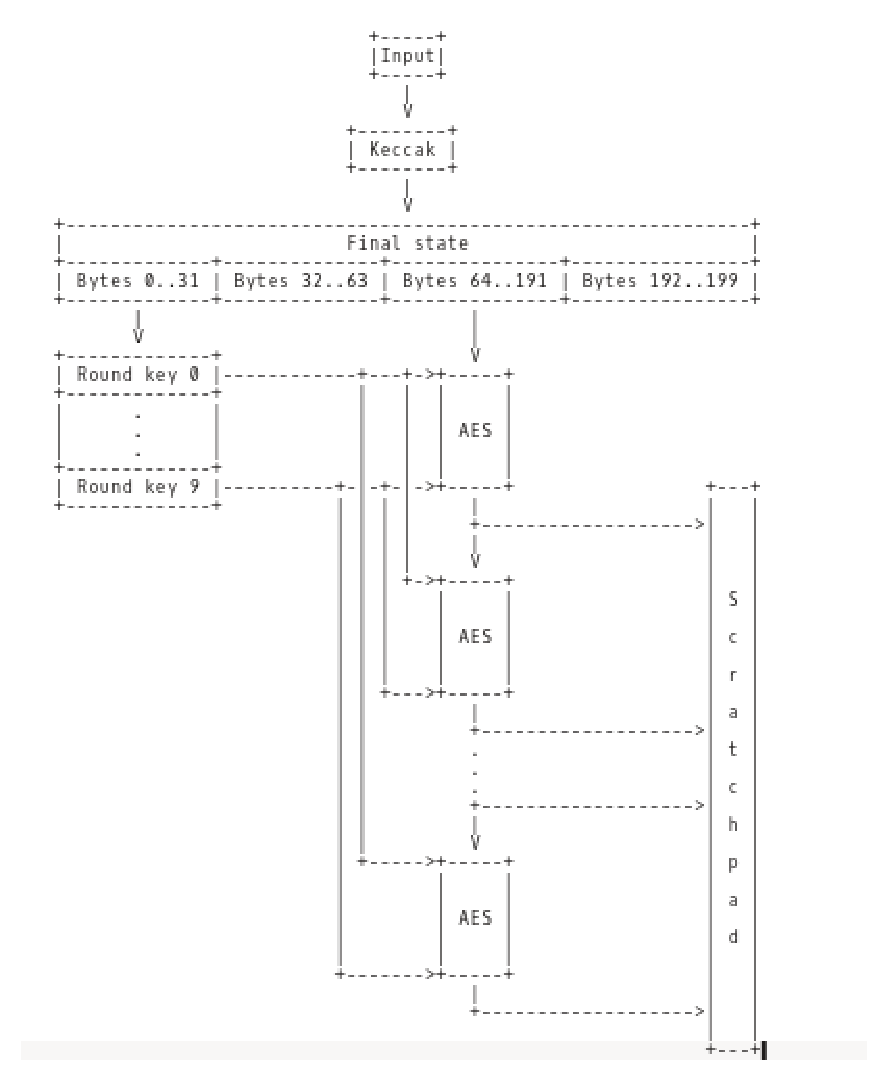
\includegraphics[width=0.6\textwidth]{monero_mining_scratchpad_init.eps}
    \caption{The Scratchpad Initialisation of the Monero Mining Process}
    \label{fig:monero_mining_scratchpad_init}
\end{figure}

\subsubsection{Memory-hard Loop}

The memory-hard loop (the main loop) is an iterative process with frequent memory access to make the mining process memory-bound, which is shown in Fig.\ref{fig:monero_mining_main_loop}.

\begin{figure}[h]
    \centering
    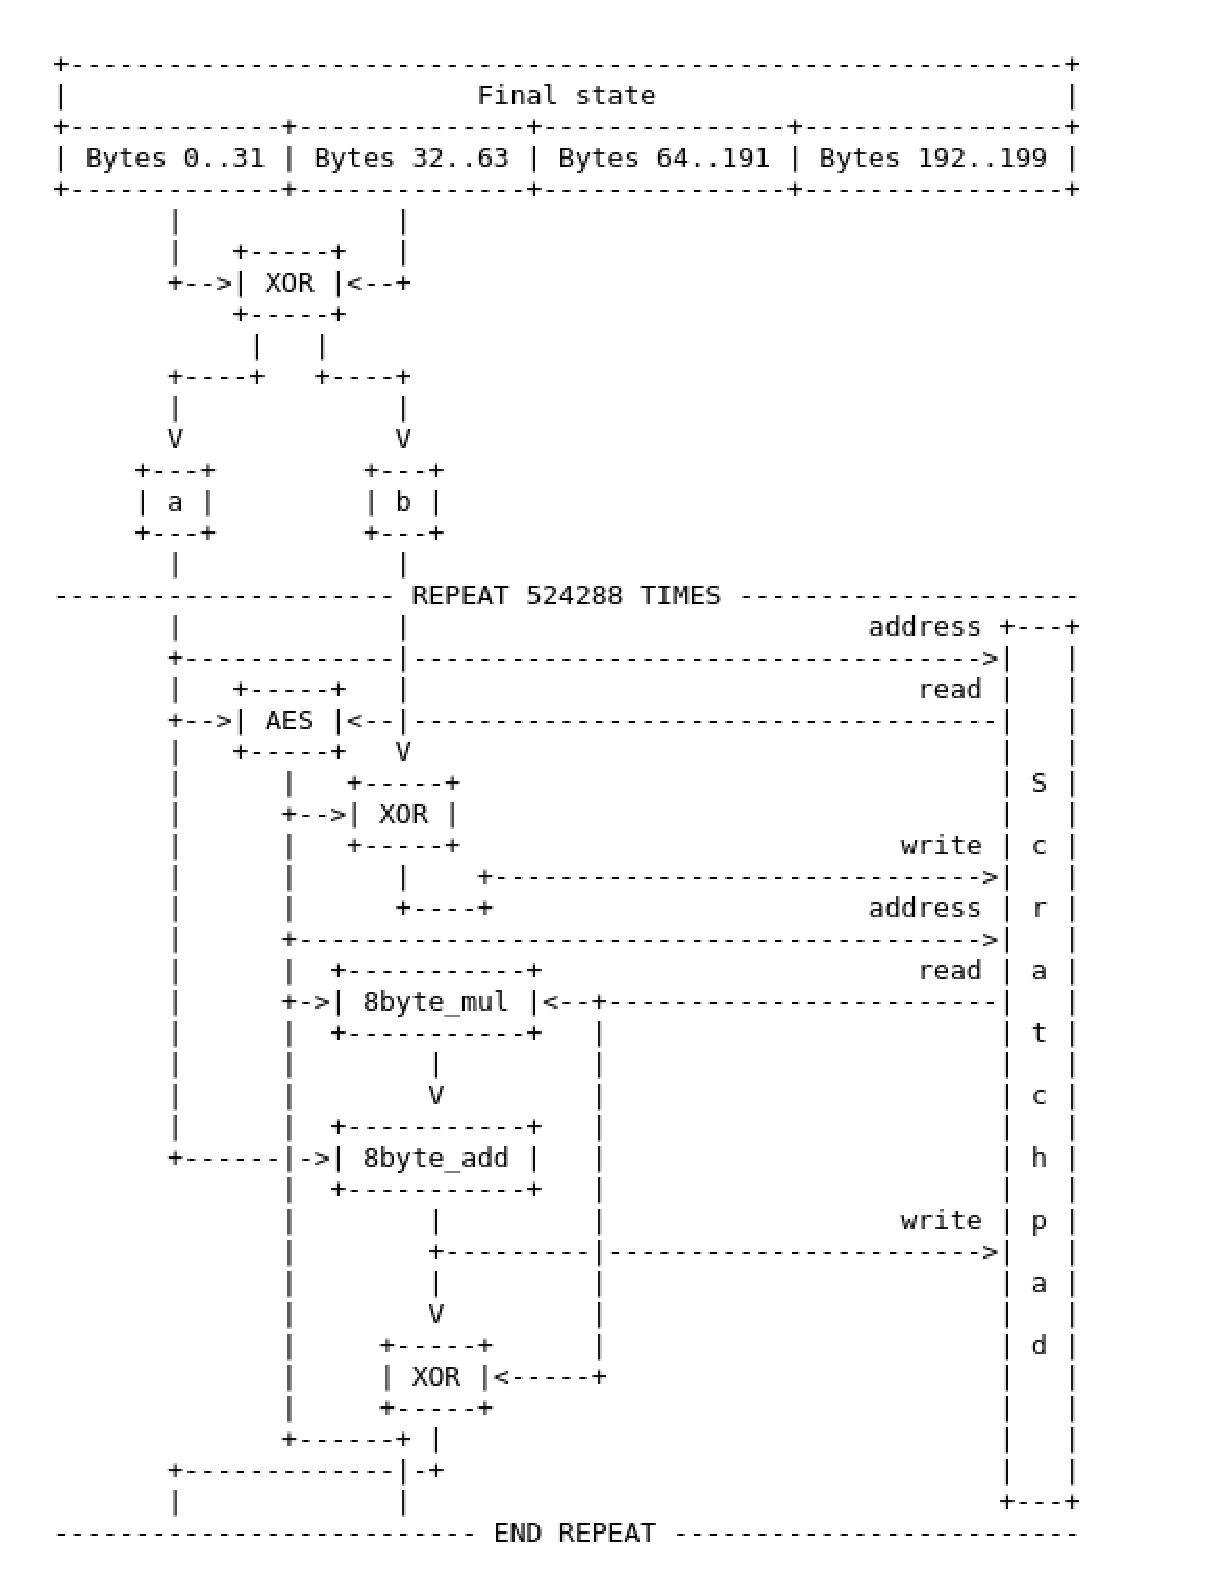
\includegraphics[width=0.6\textwidth]{monero_mining_main_loop.eps}
    \caption{The Memory-hard Loop of Monero Mining Process}
    \label{fig:monero_mining_main_loop}
\end{figure}

\subsubsection{Result Calculation}

After the memory-hard loop, the result is calculated as shown in Fig.~\ref{fig:monero_mining_result_calc}.

\begin{figure}[h]
    \centering
    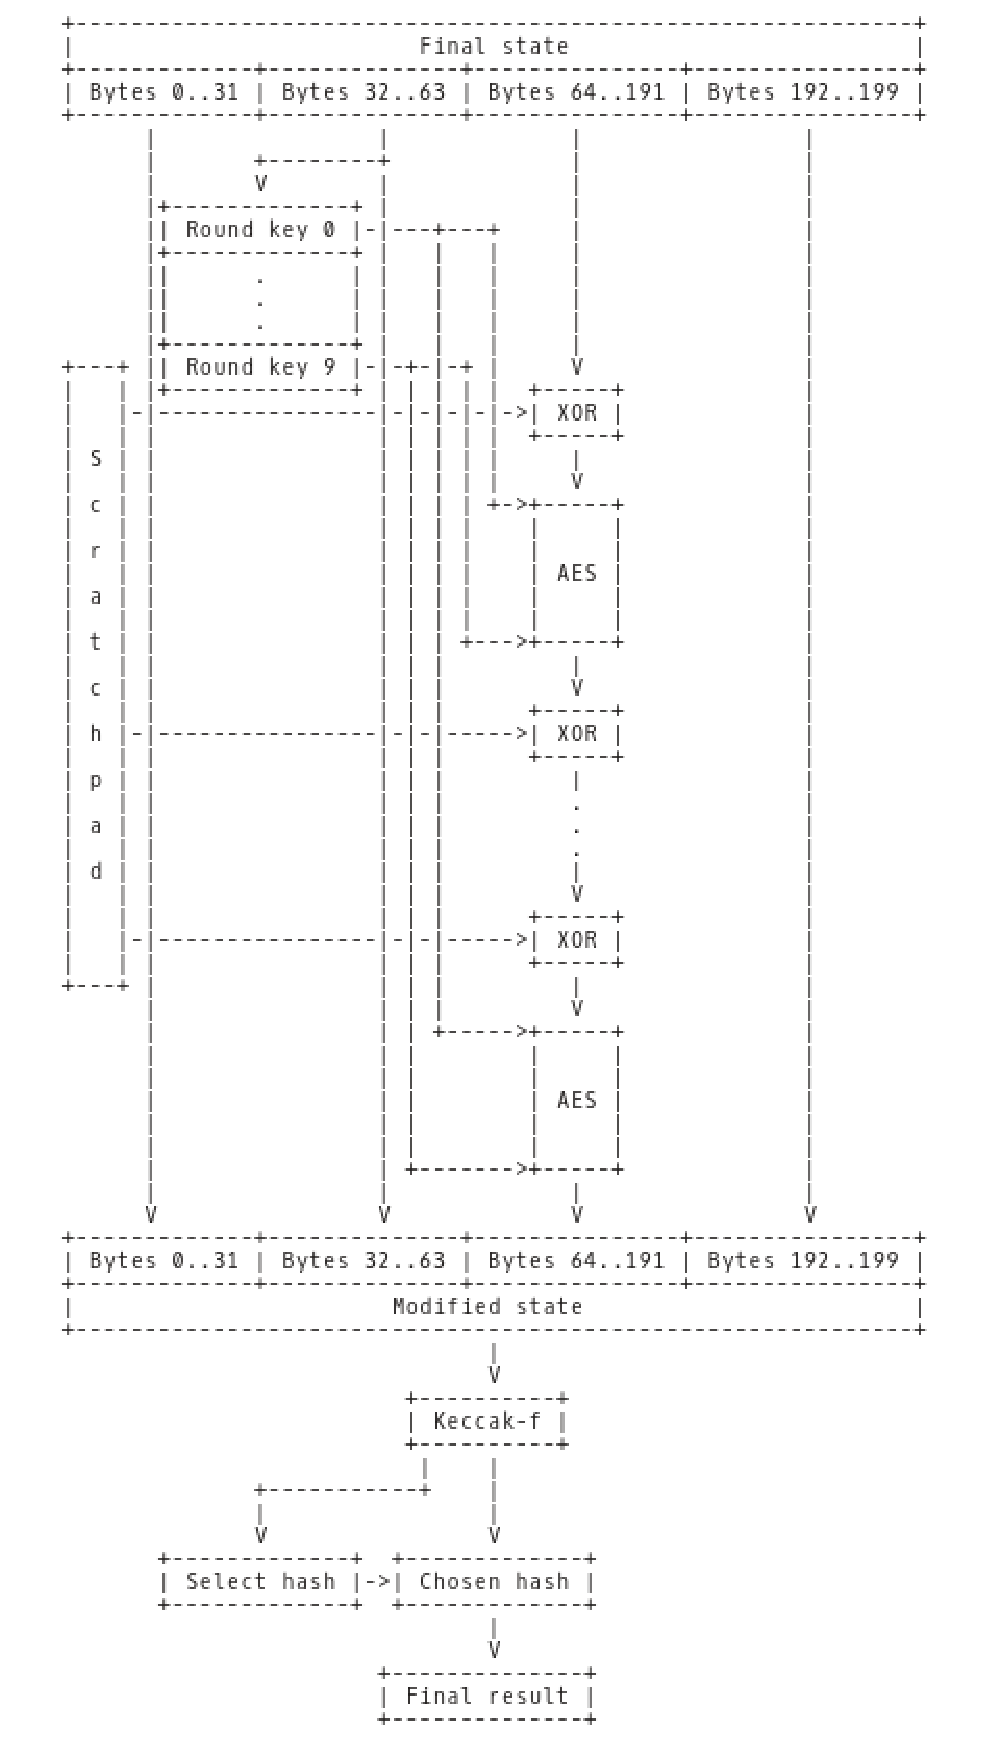
\includegraphics[width=0.6\textwidth]{monero_mining_result_calc.eps}
    \caption{The Result Calculation of Monero Mining Process}
    \label{fig:monero_mining_result_calc}
\end{figure}

\subsection{Scrypt}

Scrypt\cite{percival2016scrypt} is defined as Fig.~\ref{fig:scrypt_process}, where MF is a pluggable sequential memory-hard function.

\begin{figure}[h]
    \centering
    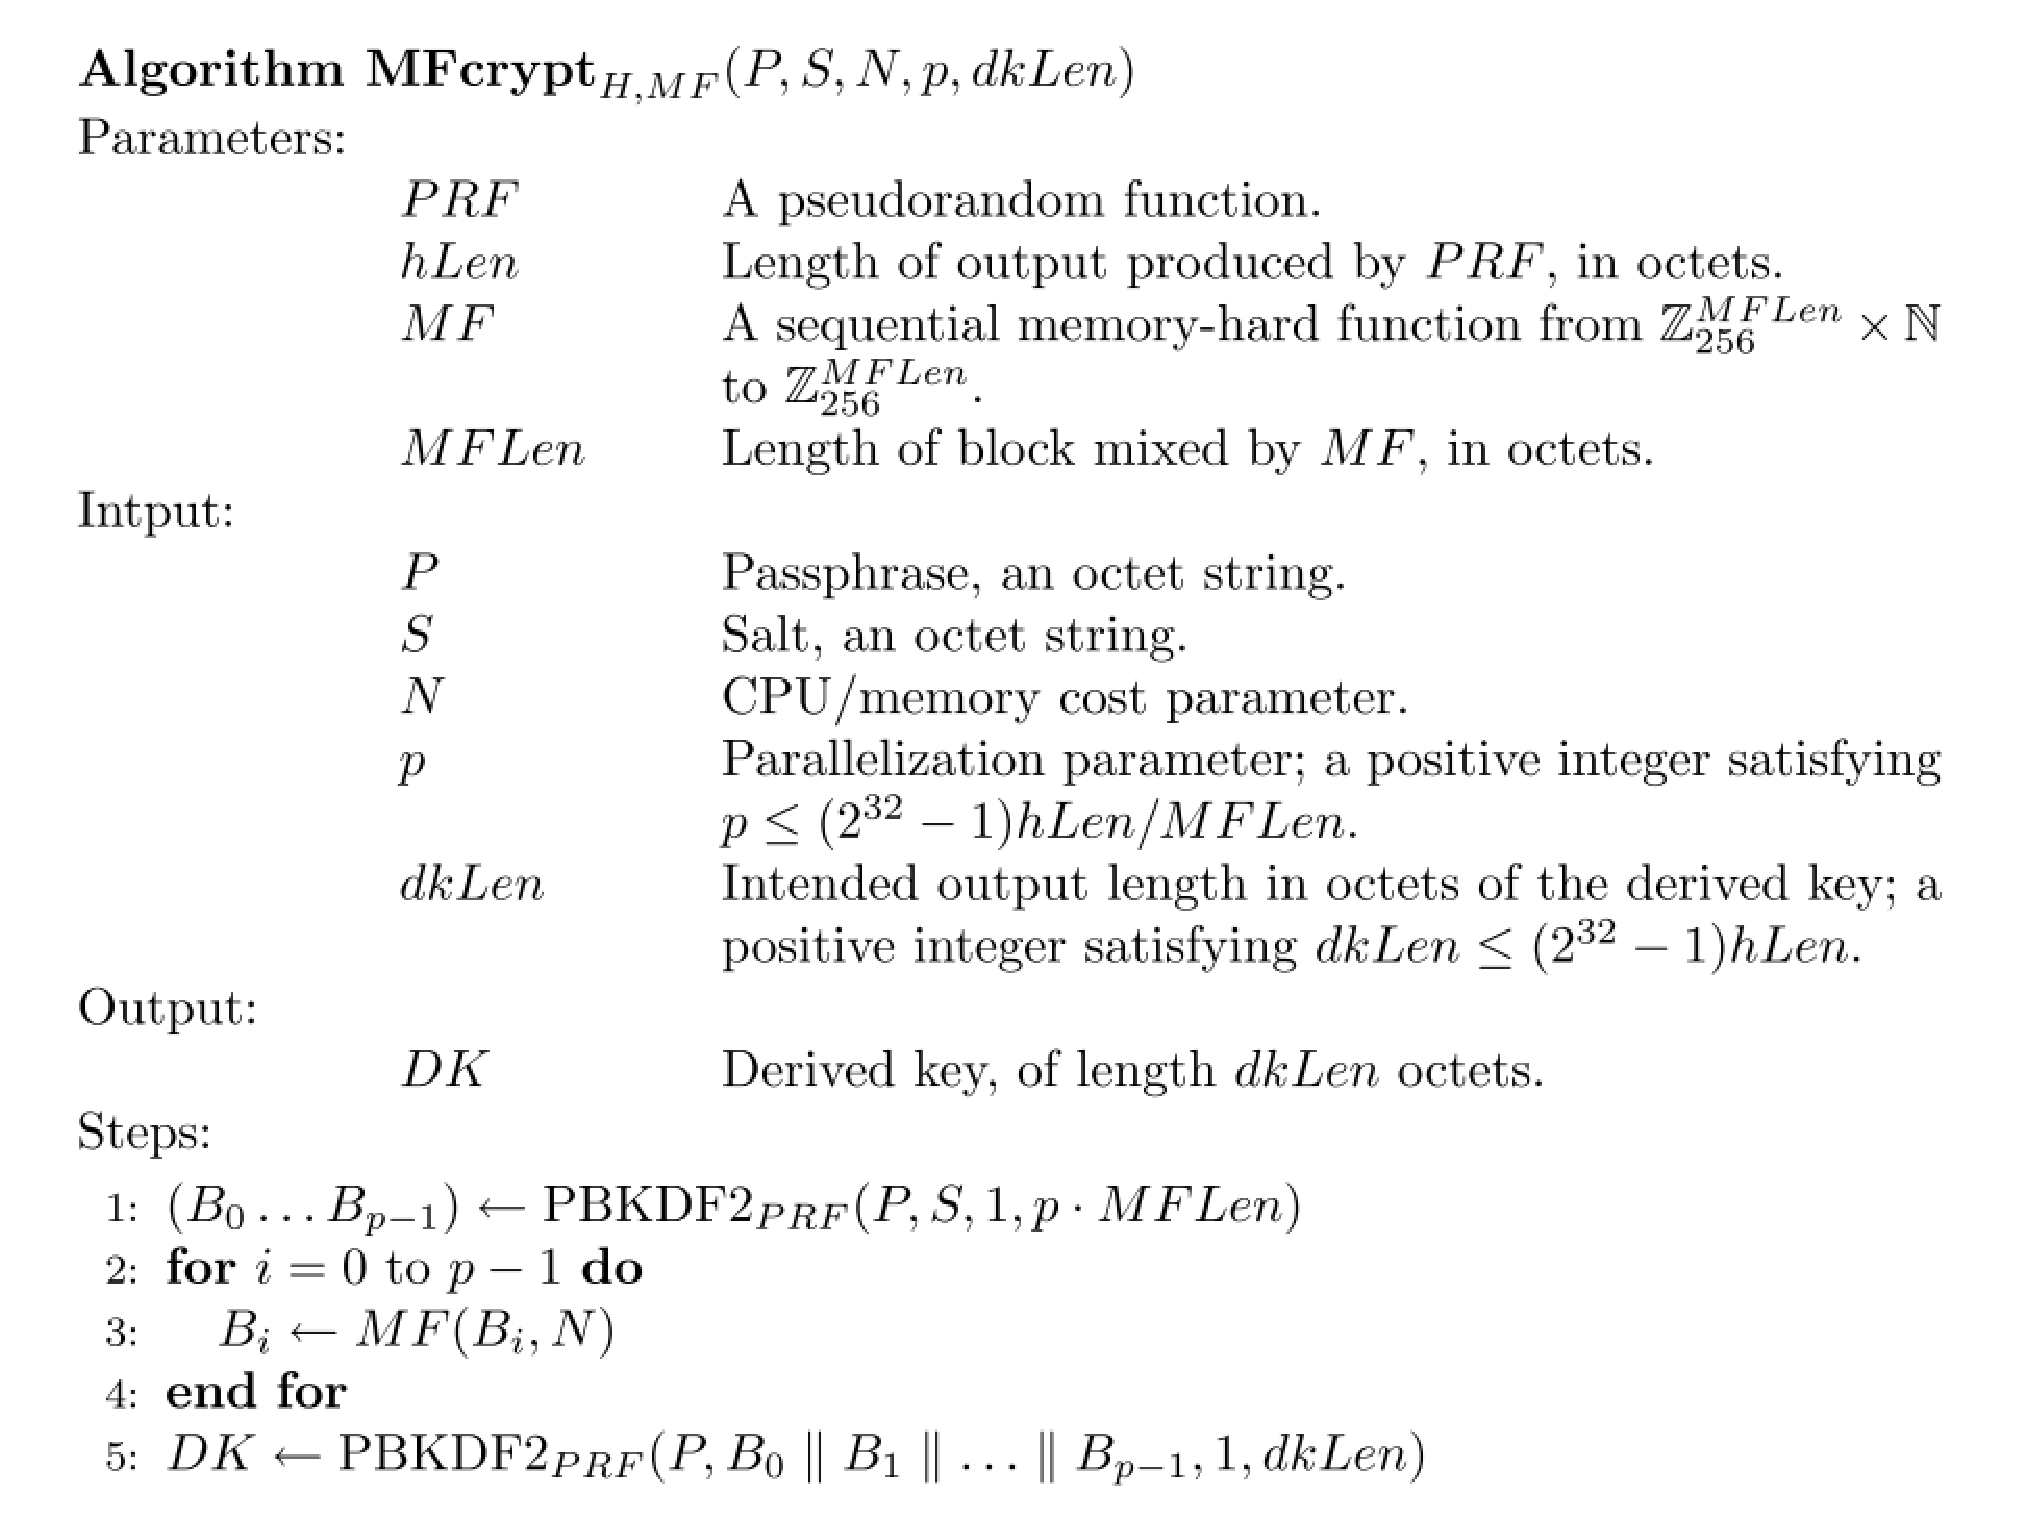
\includegraphics[width=0.6\textwidth]{scrypt_process.eps}
    \caption{The Scrypt Function}
    \label{fig:scrypt_process}
\end{figure}

PBKDF2\cite{percival2016scrypt} is the abbreviation of Password-Based Key Deviation Function 2, which takes a string and a Pseudo Random Function (PRF) as inputs and outputs a key (no need to be sequential or memory-hard).

The chosen MF is the SMix function family proposed by the Scrypt paper. An implementation of SMix functions is called $BlockMix$, the process of which is shown in Fig.~\ref{fig:scrypt_smix}.

\begin{figure}[h]
    \centering
    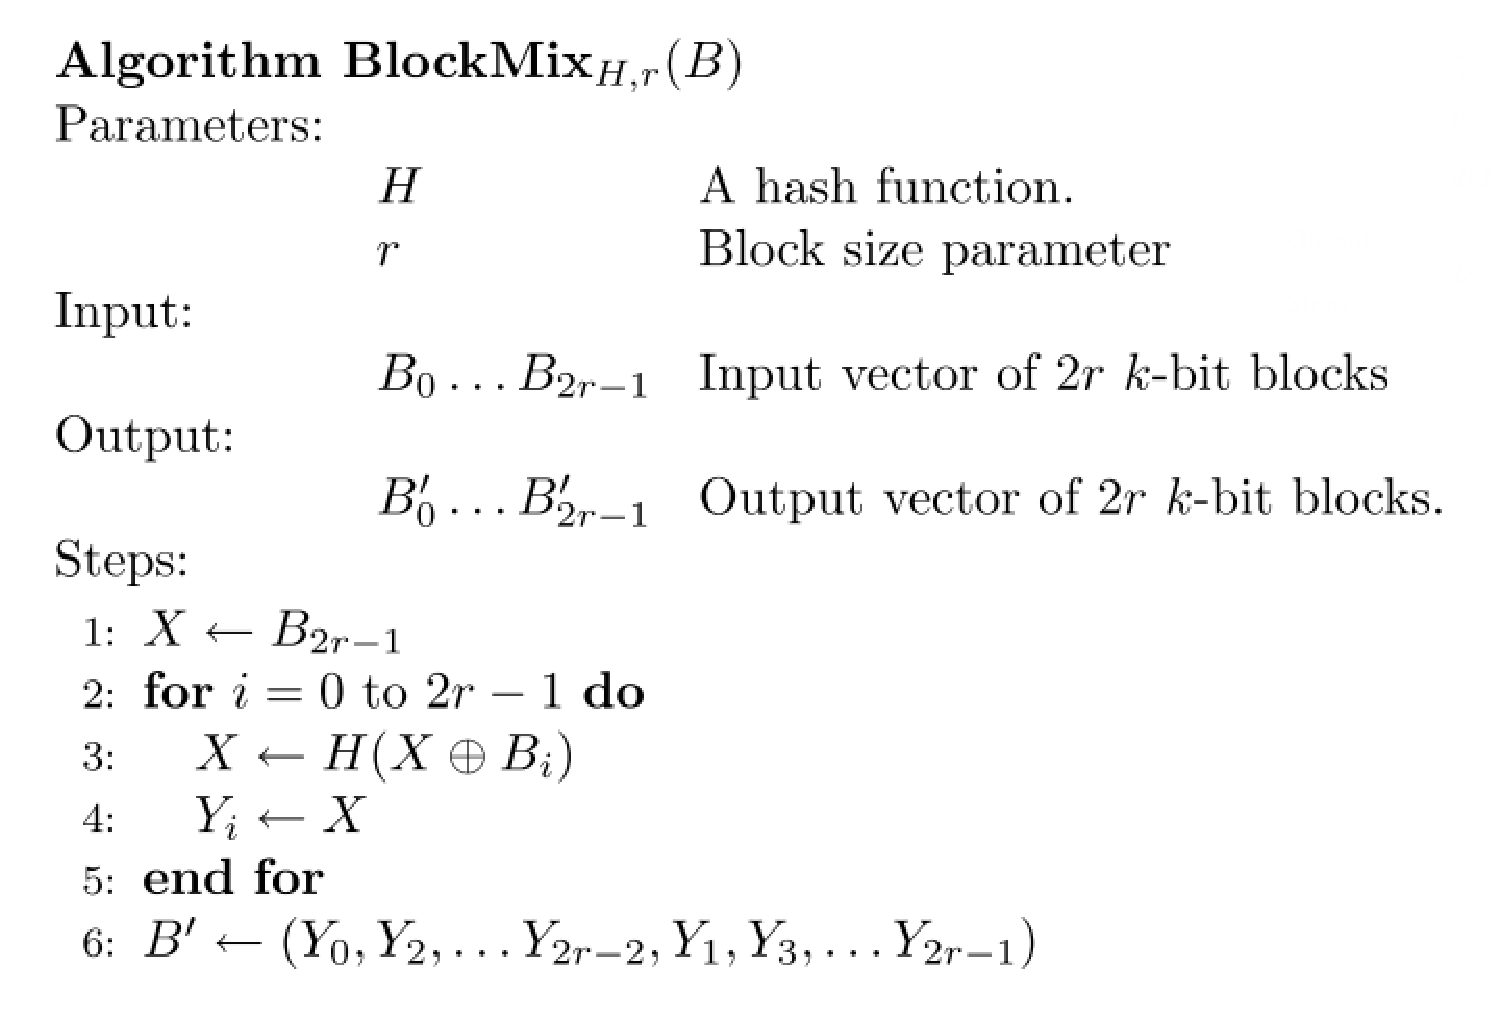
\includegraphics[width=0.6\textwidth]{scrypt_smix.eps}
    \caption{The process of BlockMix, which is a type of SMix}
    \label{fig:scrypt_smix}
\end{figure}

\section{Testing and Performance Analysis}
%TODO Testing 
%TODO performance analysis(curve)

\subsection{Ethash}

The chosen Ethash implementation is \texttt{Ethminer}\footnote{Ethminer: https://github.com/ethereum-mining/ethminer}, which is the official mining software for Ethereum with CUDA and OpenCL support. 

The benchmark result of the Ethash CUDA implementation is shown in Fig.~\ref{fig:ethash_cuda_test}, while the OpenCL implementation is shown in Fig.~\ref{fig:ethash_opencl_test}. The benchmark process is to generate the whole DAG first, then test the hashrate for five times, finally get the results and make statistics.

According to the testing, the CUDA version performs better than the OpenCL version. This is because OpenCL targets at implementing a general-purpose parallel computing platform, which inevitably causes poorer performance.

According to the statistics about the cryptocurrency market, Ethereum is the second most popular cryptocurrency combined with state-of-the-art features Bitcoin does not have, like the memory-bound Ethash mining, the Smart Contract and the new Zero Knowledge Proof privacy protection. It is reasonable to put the Ethash in a high priority.

\begin{figure}[h]
    \centering
    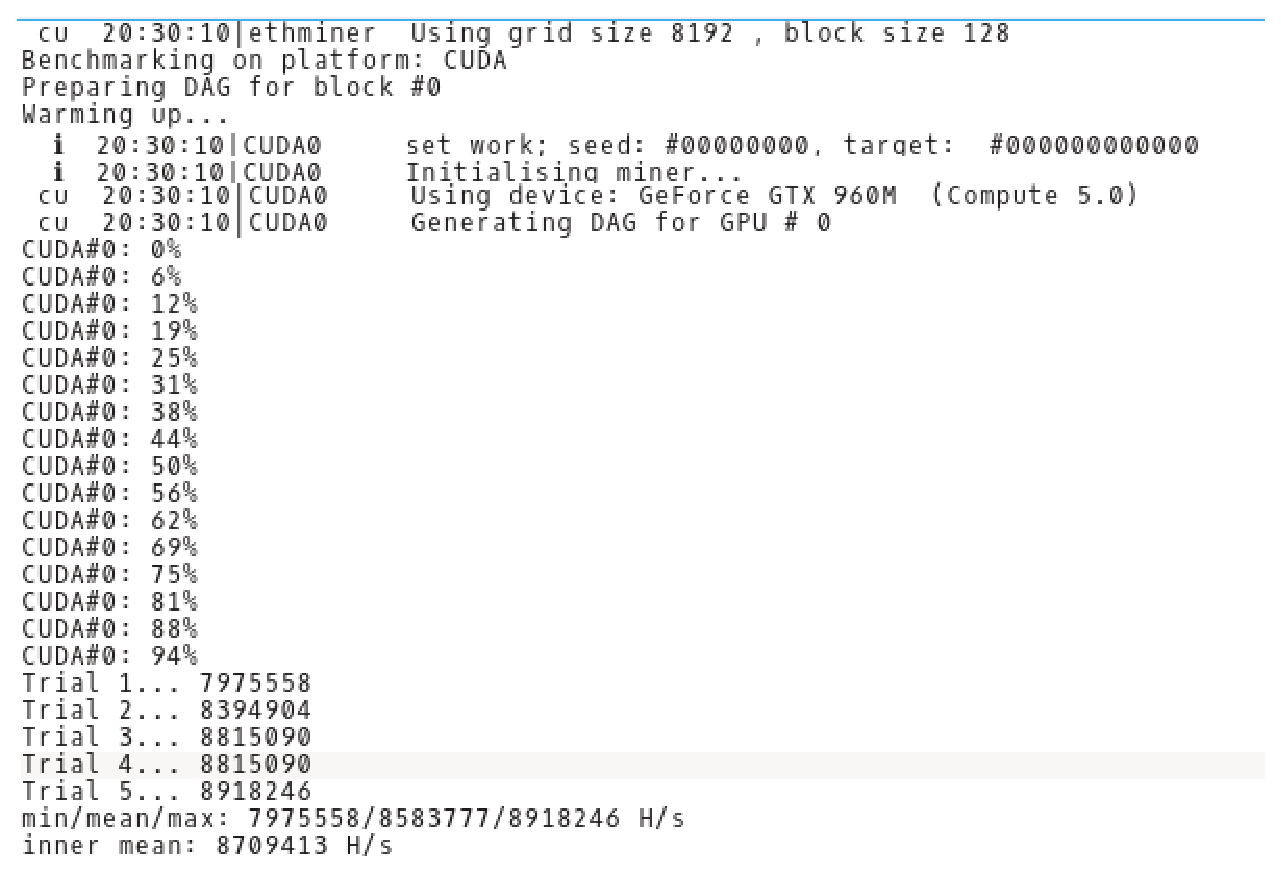
\includegraphics[width=0.6\textwidth]{ethash_cuda_test.eps}
    \caption{The benchmark result of the Ethash CUDA implementation}
    \label{fig:ethash_cuda_test}
\end{figure}

\begin{figure}[h]
    \centering
    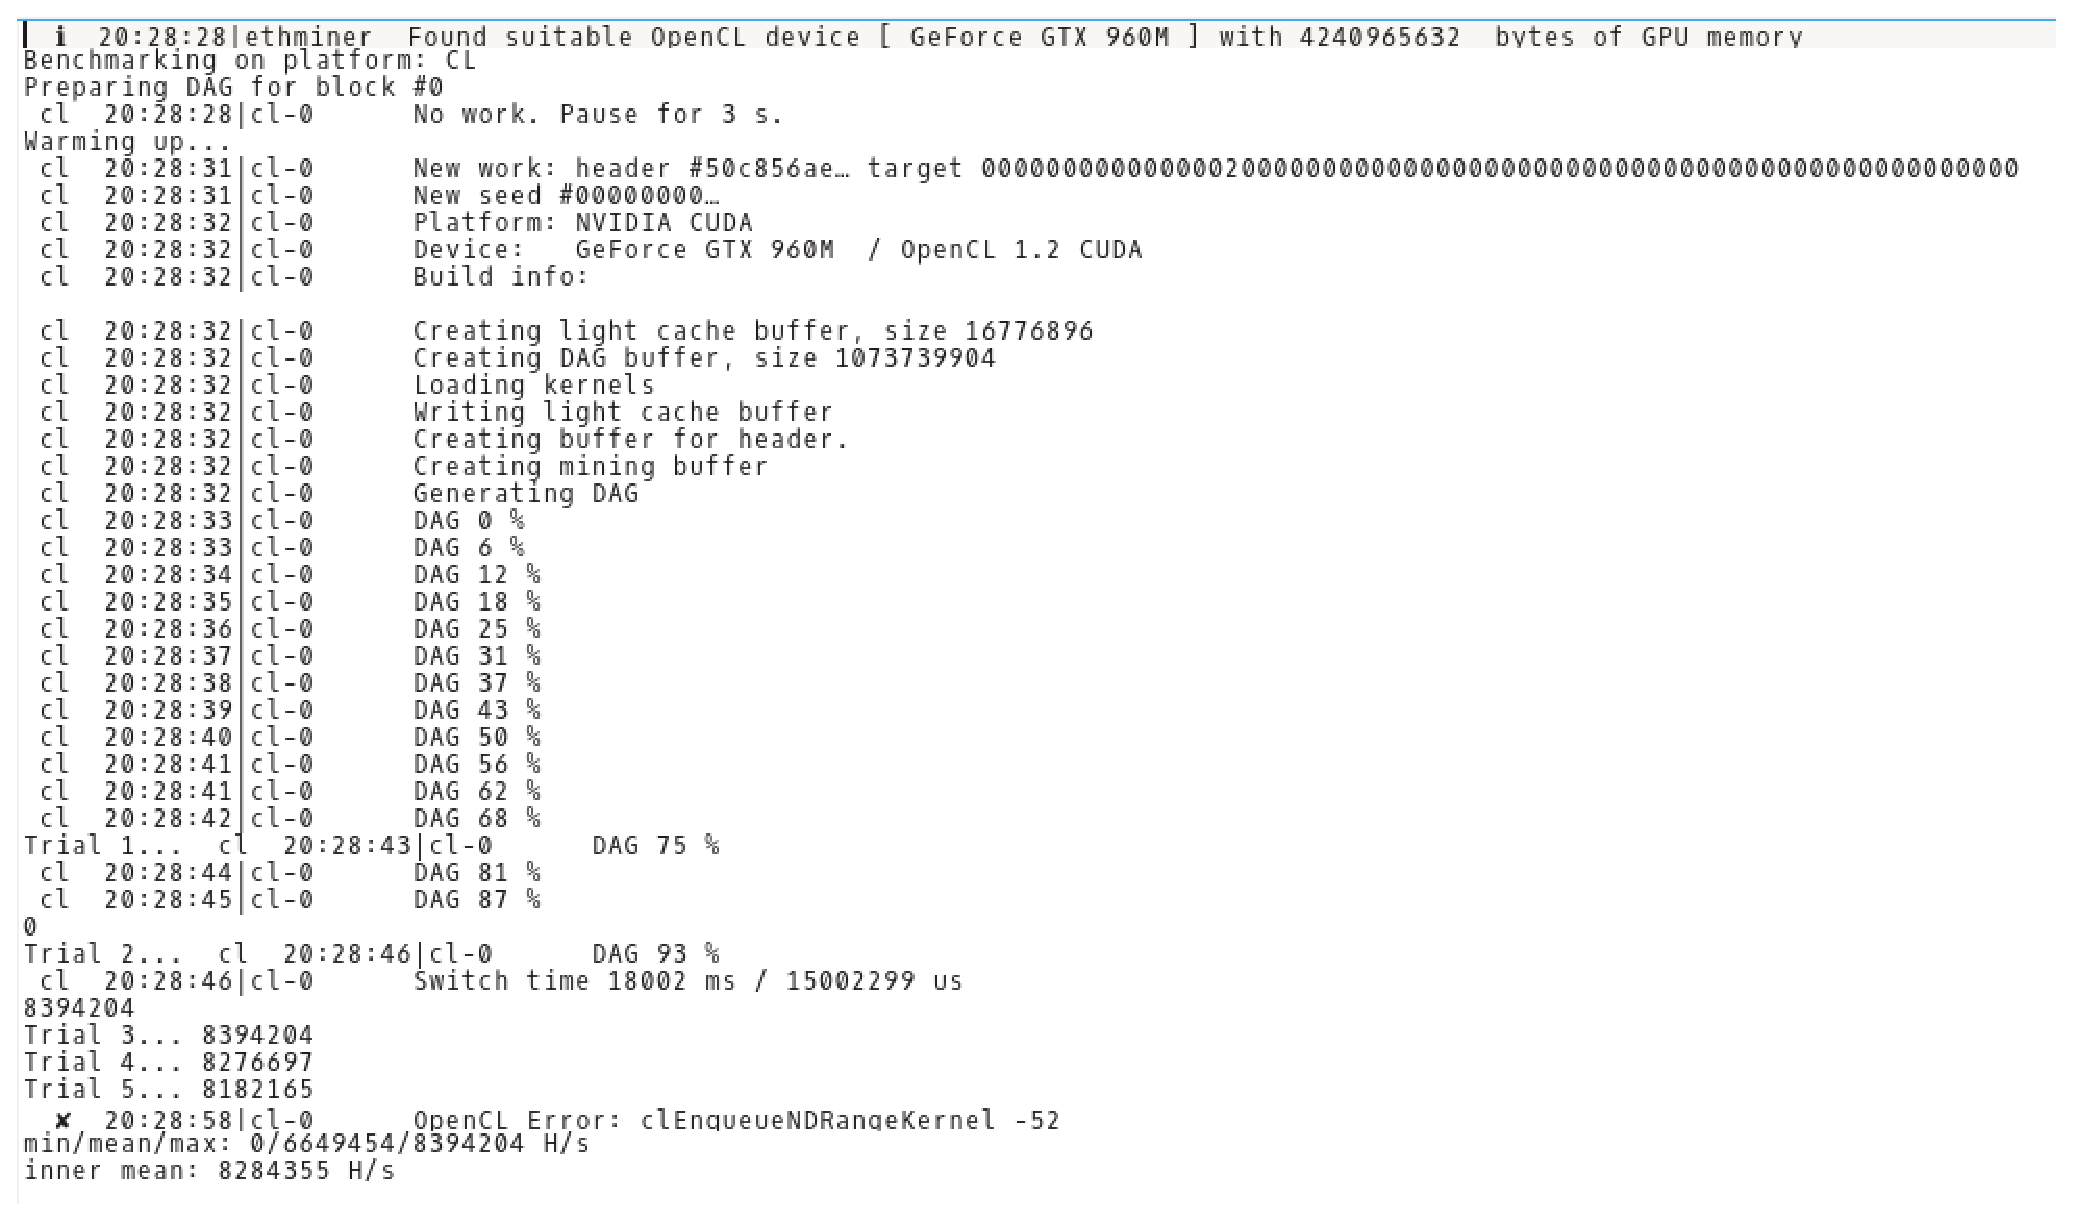
\includegraphics[width=0.6\textwidth]{ethash_opencl_test.eps}
    \caption{The benchmark result of the Ethash OpenCL implementation}
    \label{fig:ethash_opencl_test}
\end{figure}



\subsection{Scrypt}

The \texttt{ccminer} implementation of Scrypt CUDA is chosen, where \texttt{ccminer} is a miner supporting a wide range of mining algorithms\footnote{ccminer: https://github.com/cbuchner1/ccminer}. It is noted that the Scrypt performance is much poorer than Ethash. This is because Scrypt is unparallelisable but Ethash is parallelisable, while both of them are memory-bound.

\begin{figure}[h]
    \centering
    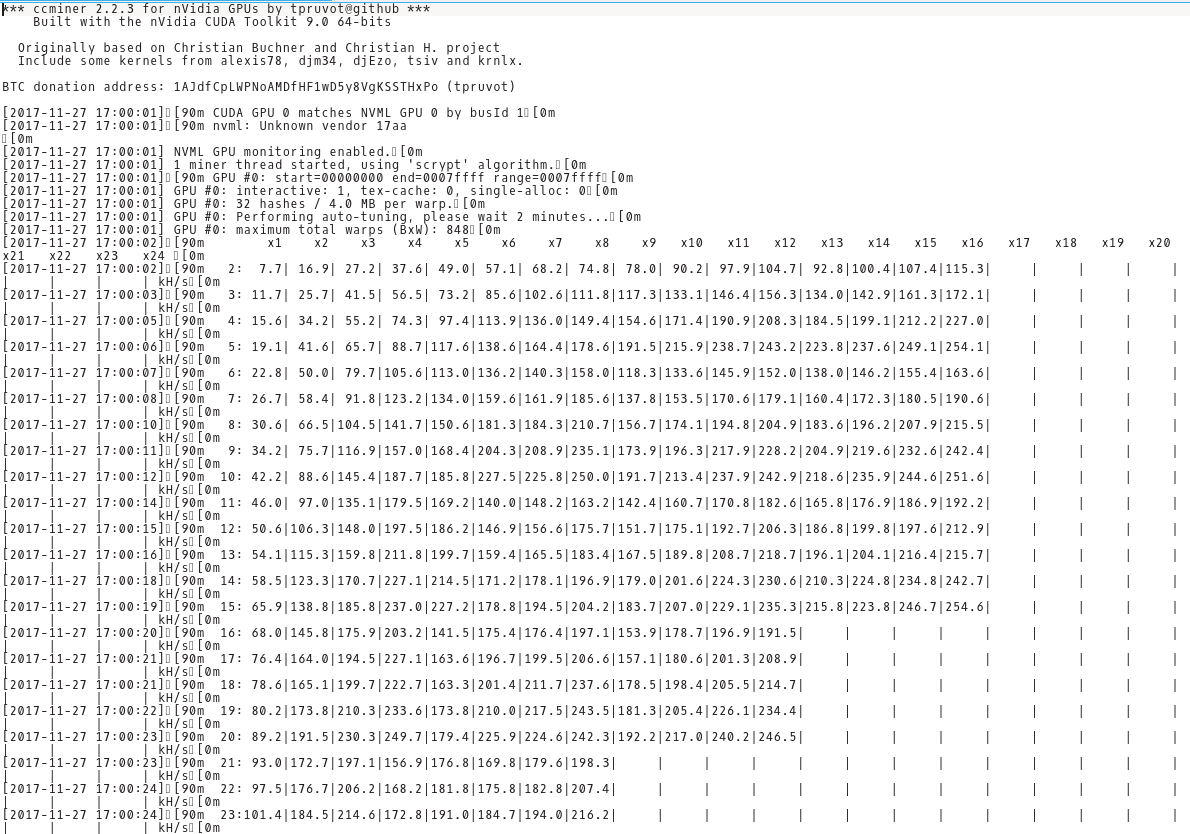
\includegraphics[width=0.6\textwidth]{scrypt_cuda_test1.eps}
    \caption{The benchmark result of the Scrypt CUDA implementation 1}
    \label{fig:scrypt_cuda_test1}
\end{figure}

\begin{figure}[h]
    \centering
    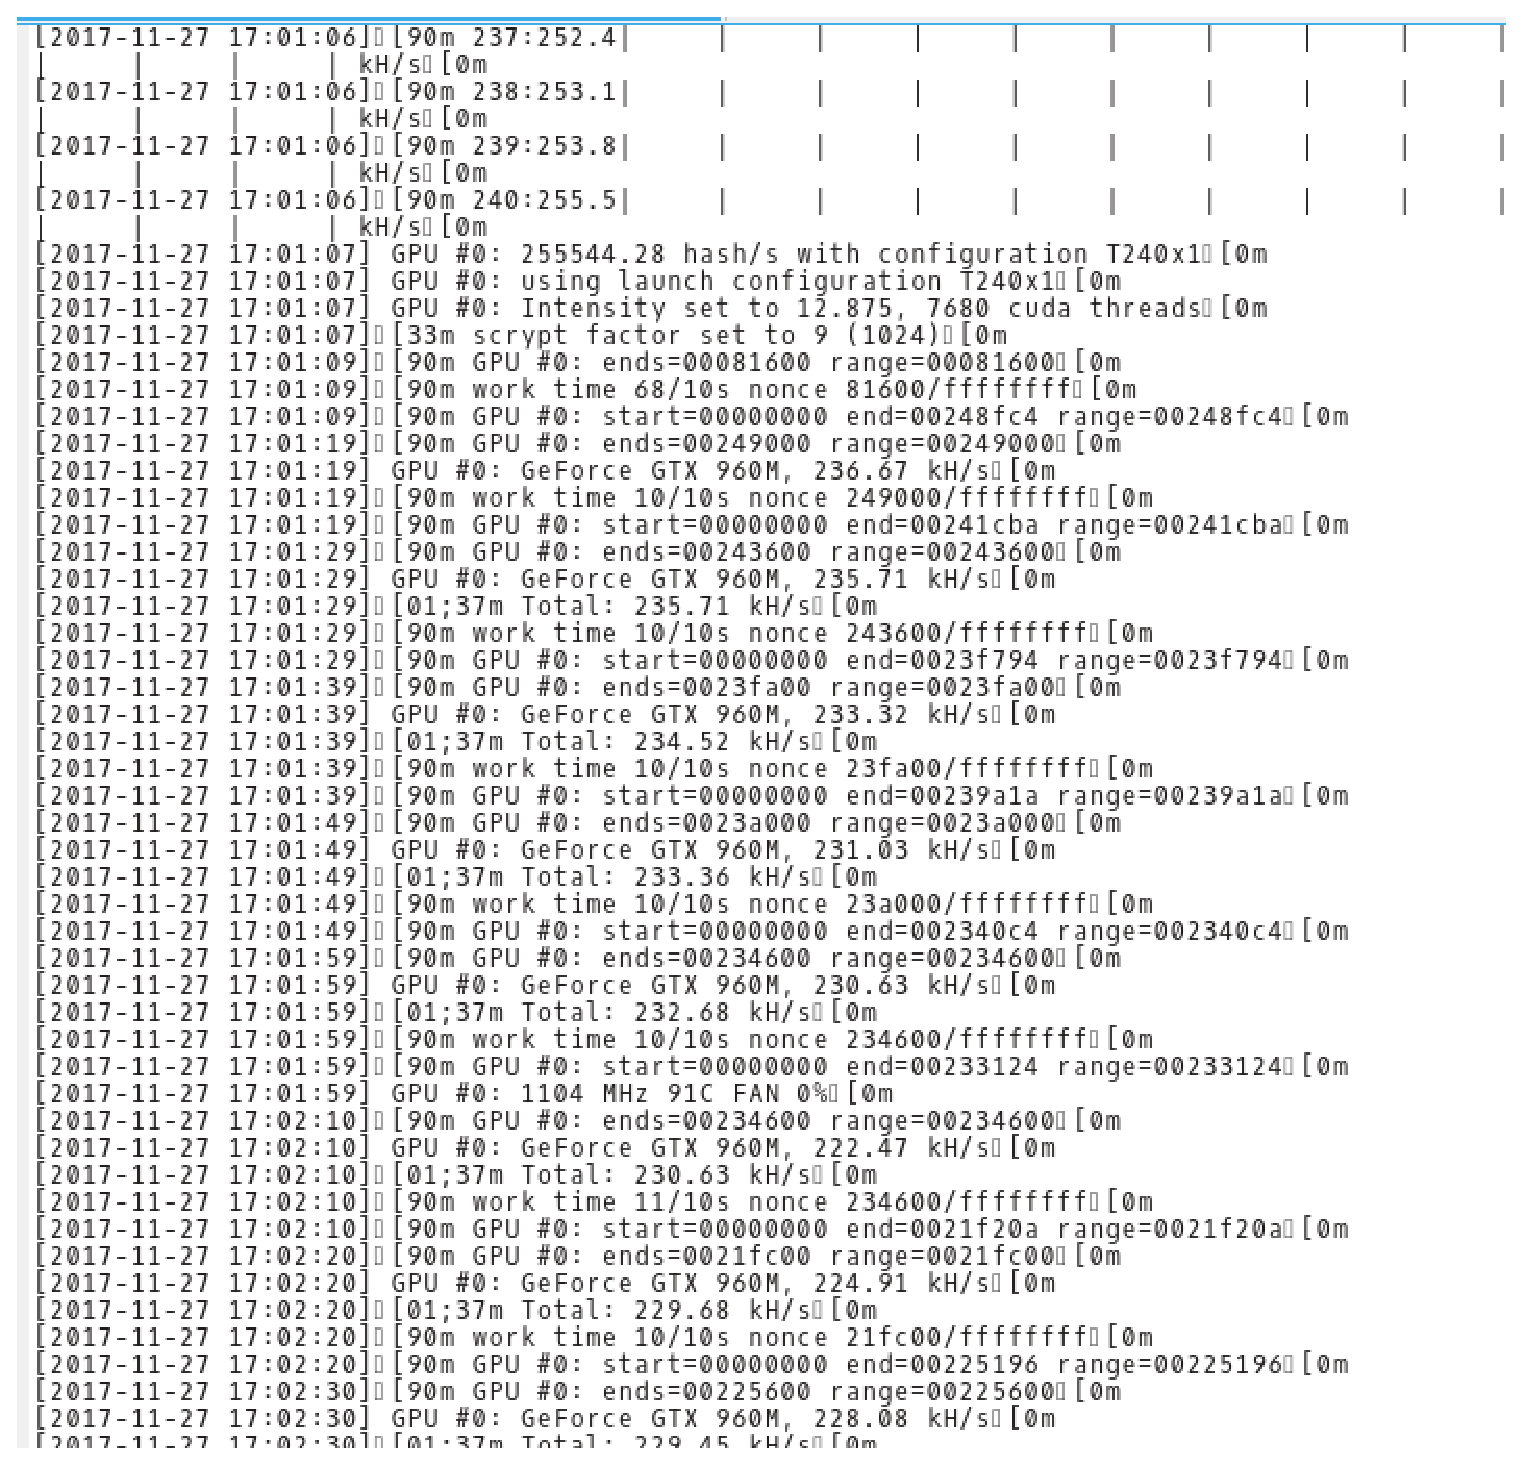
\includegraphics[width=0.6\textwidth]{scrypt_cuda_test2.eps}
    \caption{The benchmark result of the Scrypt CUDA implementation 2}
    \label{fig:scrypt_cuda_test2}
\end{figure}


\subsection{CryptoNight}

\texttt{ccminer} has the CryptoNight CUDA implementation, too. However, unfortunately when I tried to run it, my computer crashed and rebooted. The next step is to limit its GPU usage and run again.

\section{Miscellaneous}

\begin{itemize}
\item Deleted the Cuckoo algorithm because it is not widely used, but added Cryptonight of Monero
\end{itemize}
%
% This section is used to list the following week's plan
% Use the \item construct to list each item.  Try to keep the
% Descriptions for each down to one or two sentences
%
\section{Next Week's Plan}
\begin{itemize}
\item Benchmark chosen algorithms with specified parameters(in hardware simulators?)
\item Try to understand source code of chosen algorithms
\item Learn CUDA programming and other related tools 
\end{itemize}

\bibliographystyle{plain}
\bibliography{references.bib}

\end{document}
